\chapter{\label{ch:methodology} Methodology}
This chapter details the design and implementation of a mobile robotic system using augmented reality (AR), fiducial markers, and remote monitoring to improve human-robot interaction (HRI). It builds on existing research in computer vision-based navigation, AR for HRI, and internet-controlled mobile robots. Design decisions are justified with related literature and practical system requirements
\section{\label{sec:overview} Overview}

The high-level diagram illustrates the mobile robot project's architecture, showcasing key components: Raspberry Pi (central processor), camera module, motor control system, fiducial markers, and web-based control interface. The data flow begins with the camera capturing video, which the Raspberry Pi processes for marker detection and navigation. Simultaneously, the web interface sends commands to the Raspberry Pi, which also streams video back to the user. 

\begin{figure}[H]
    \centering
    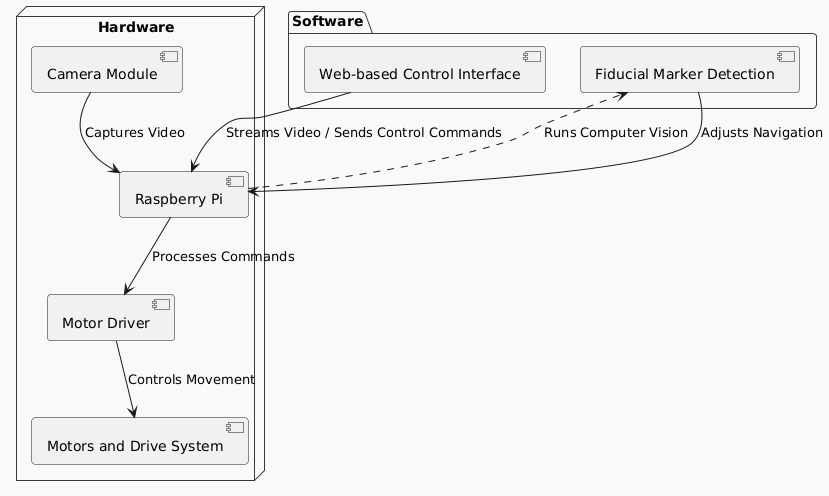
\includegraphics[width=0.7\textwidth]{ch3/figs/diagram.png}
    \caption{High Level Diagram of how the project will run}
    \label{fig:high_level_diagram}
\end{figure}

The methodology centers on the development of a mobile robot system capable of navigation, interaction, and real-time feedback, using AR markers and remote control via a Raspberry Pi board. Inspired by the works of La Delfa et al. \cite{delfa2015}, Jacobsen et al. \cite{jacobsen2018}, and Vanitha et al. \cite{vanitha2016}, this project seeks to incorporate advances in fiducial marker systems and AR interfaces to improve the efficiency and user engagement in controlling mobile robots.

